\PassOptionsToPackage{svgnames}{xcolor}
\documentclass{book}
\usepackage[utf8]{inputenc}
\usepackage{graphicx}
\usepackage{listings}
\usepackage{hyperref}
\usepackage{amsmath}
\usepackage{xcolor}

\usepackage{tcolorbox}
\tcbuselibrary{skins,breakable}
\usetikzlibrary{shadings,shadows}

\newenvironment{myexampleblock}[1]{%
    \tcolorbox[beamer,%
    noparskip,breakable,
    colback=LightGreen,colframe=DarkGreen,%
    colbacklower=LimeGreen!75!LightGreen,%
    title={#1}, width=\textwidth]}%
    {\endtcolorbox}

\newenvironment{myalertblock}[1]{%
    \tcolorbox[beamer,%
    noparskip,breakable,
    colback=LightCoral,colframe=DarkRed,%
    colbacklower=Tomato!75!LightCoral,%
    title={#1}, width=\textwidth]}%
    {\endtcolorbox}

\newenvironment{myblock}[1]{%
    \tcolorbox[beamer,%
    noparskip,breakable,
    colback=LightBlue,colframe=DarkBlue,%
    colbacklower=DarkBlue!75!LightBlue,%
    title={#1}, width=\textwidth]}%
    {\endtcolorbox}

\newcommand{\code}[1]{\mbox{% added this percent
    \ttfamily
    \tcbox[
        on line,
        boxsep=0pt, left=4pt, right=4pt, top=2pt, bottom=1.5pt,
        toprule=0pt, rightrule=0pt, bottomrule=0pt, leftrule=0pt,
        oversize=0pt, enlarge left by=0pt, enlarge right by=0pt,
        colframe=white, colback=black!12,
        height=.8\baselineskip % added this (and guessed at .8)
    ]{#1}% added this percent
}}


\newtheorem{definition}{Definition}


\begin{document}
\setlength{\parindent}{0cm}
\chapter{Git and GitHub}

intro

Explain what git and GitHub are and their purposes

dépôt au lieu de repository/repo dans ce tutoriel

\section{Config}

Cette section devrait déjà être faite, vous devriez déjà avoir un compte github, avoir téléchargé git et avoir configuré votre email. Si jamais ce n'est pas fait, voici comment le faire. 

Commencez par ouvrir votre terminal et taper "git" 

\begin{figure}[!h]
    \centering
    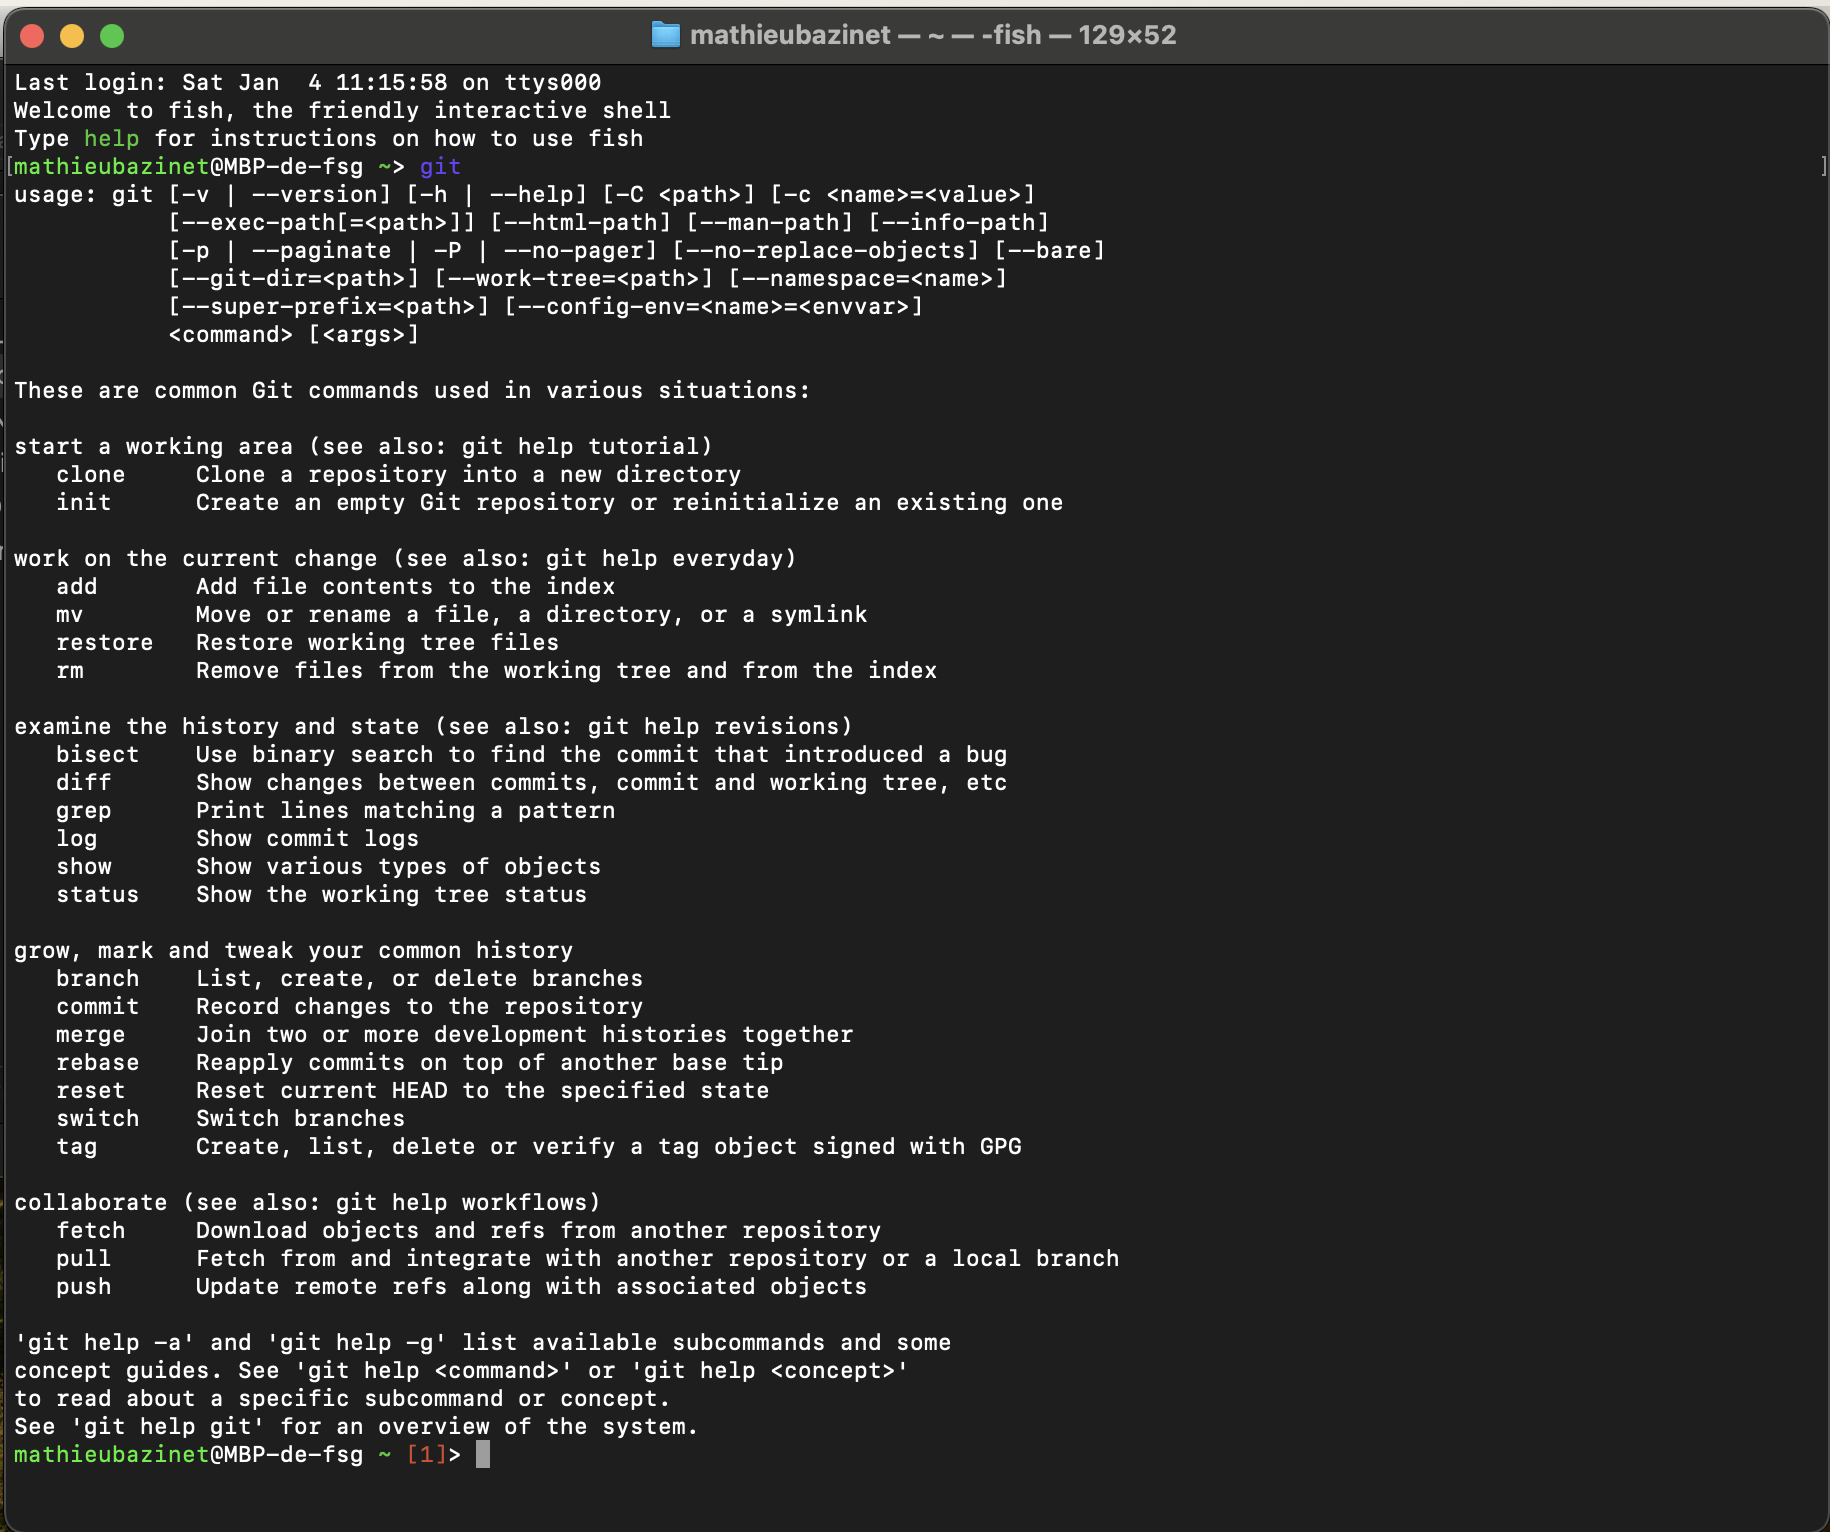
\includegraphics[width=0.8\textwidth]{images/check_if_git.png}
    \caption{Sortie attendue dans le terminal lorsque la commande ``git'' est tapée dans le terminal.} \label{fig:check_if_git}
\end{figure}
Download : 
	\url{https://git-scm.com/}
	xcode-select --install

Configuring git :
\begin{lstlisting}
	git config --global user.email "votre_courriel@ulaval.ca"
	git config --global user.name "votre_nom"
\end{lstlisting}
token d’identification (Mac) (\url{https://docs.github.com/fr/authentication/keeping-your-account-and-data-secure/managing-your-personal-access-tokens\#cr%C3%A9ation-dun-personal-access-token-classic}) 



\section{Première étape avec Git}

Cloner le repo de ce tutoriel
aller chercher le lien du repo

\begin{figure}[!h]
    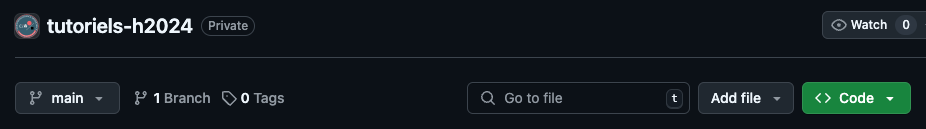
\includegraphics[width=\textwidth]{images/clone_button_github.png}
    \caption{À remplir} \label{fig:clone_button}
\end{figure}

cloner un repo

\begin{myexampleblock}{Exercice : Clôner le dépôt du tutoriel}
Vous allez maintenant cloner le dépôt Git du tutoriel.

\texttt{git clone https://github.com/cia-ulaval/tutoriels-h2024.git}

\end{myexampleblock}



\begin{myblock}{git clone}
    La commande \texttt{git clone <url-du-repo>} permet de créer une copie locale du projet. 
\end{myblock}

Normalement, un bon repo va avoir les quatre fichiers suivants : 
\begin{enumerate}
    \item README.md
    \item LICENSE
    \item .gitignore
    \item requirements.txt
\end{enumerate}

\subsection{README}
\url{https://www.freecodecamp.org/news/how-to-write-a-good-readme-file/}
Le README est le premier contact entre l'utilisateur et le dépôt. C'est un fichier markdown qui doit donner les informations nécessaires à utiliser le code du dépôt. Le README va contenir un titre, 

Project's title
Project description
How to install the project/ en lien avec le requirements.txt + la version de Python si applicable

How to use the project (quels fichiers font quoi, si c'est des expériences dans un papier, comment rouler les expériences, etc. )

Crédits, si du code provient d'un autre endroit, le nom des collaborateurs, sources, etc. 
contact information
\subsection{LICENSE}

S'il n'y a pas de license, c'est équivalent à "ne pas toucher". Il y a beaucoup de chercheurs qui ne mettent pas de license en se disant que ça devient "open-source" et peut-être utilisé par n'importe qui, mais c'est le contraire. Pas de license veut dire que tous les droits sont à l'auteurs et que tu ne peux pas utiliser le code. Dans un petit projet, ce n'est pas très grave, personne va vous taper sur les doigts. Si vous faites de la recherche/ vous voulez publier du code et laisser la communauté l'utiliser, il faut demander la permission aux auteurs ou suivre la license. 

Les licenses les plus classiques
CC-BY 4.0 
MIT
Licence publique générale GNU v3.0
Licence Apache 2.0

\url{https://choosealicense.com/no-permission/}
\url{https://choosealicense.com/}
\url{https://docs.github.com/fr/repositories/managing-your-repositorys-settings-and-features/customizing-your-repository/licensing-a-repository}


\subsection{.gitignore}
Le fichier gitignore n'est pas le fichier le plus intéressant. C'est purement un fichier utilitaire. Il va être utile uniquement si l'utilisation de votre code crée des fichiers qui ne doivent pas se retrouver sur github. Par exemple, si votre code télécharge MNIST, on ne veut pas qu'il se retrouve sur GitHub. De plus, directement dans le dossier Tuto1-GitHub, vous trouverez un fichier ``.tex''. Si vous compilez le fichier, vous aurez un pdf ainsi que des fichiers avec des extensions tels que ".aux", ".fls", ".log", ".out", etc. Ces fichiers ne sont pas pertinents, et je ne veux pas oublier de les enlever et mettre des fichiers inutiles sur github. Si vous regardez le fichier .gitignore, vous verrez en bas les lignes suivantes : 

\begin{lstlisting}
*.aux
*.fdb_latexmk
*.fls
*.out
*.synctex.gz
\end{lstlisting}

Vous ne les trouverez pas sur GitHub, puisqu'ils sont automatiquement ignorés. L'astérisque au début veut dire : tous les fichiers de style nom\_du\_fichier.aux va être matché par *.aux. 

\url{https://git-scm.com/docs/gitignore}


\subsection{requirements.txt}
En plus de la version de Python donnée dans le README, il est de bonne usage de donner la version des librairies utilisées par le projet. Vous garantissez que le code va fonctionner et sera reproductible si l'utilisateur utilise la version des librairies que vous avez utilisés. 

pip freeze $>$ requirements.txt
pip install -r requirements.txt


\section{Créer un dépôt Git}\label{sec:creer_depot}

Techniquement, il est possible de créer un dépôt avec \texttt{git init}. Je trouve qu'il est beaucoup plus facile de le faire directement sur GitHub. Vous devrez choisir : 

un nom
Description courte
Si le repo est privé ou public
Ajouter un README
Ajouter un gitignore
Choisir une licence

\textcolor{red}{Dans la section sur comment créer un repo, Parler des repo <Nom-d'utilisateur> et <nom-d'utilisateur>.github.io }

\url{https://github.com/MathieuBazinet}
contient uniuqmenet un readme qui va être display

\url{https://github.com/MathieuBazinet/MathieuBazinet.github.io}
contient le contenu qui va se retrouver dans le site web.
\url{https://mathieubazinet.github.io/fr/}

\url{https://github.com/NathanielDamours} un repo sans readme

\begin{myexampleblock}{Exercice : Créer un dépôt Git}
Dans cet exercice, vous allez créer un dépôt Git. 
\begin{enumerate}
    \item Sur GitHub, créez un nouveau dépôt en cliquant sur le bouton vert ``New''.
    \item Choisissez le nom du dépôt. Nous recommandons ``tuto-cia'' ou d'utiliser le nom aléatoire généré par GitHub. 
    \item Ajoutez une petite description du dépôt. 
    \item Cliquez sur ``Private'' pour créer un dépôt privé.
    \item Ajoutez un README
    \item Choisissez le .gitignore de votre choix en tapant le langage de programmation que vous utilisez. 
    \item Choisissez une licence de votre choix. Je recommande ``MIT License''.
    \item Créez votre dépôt.
\end{enumerate}
\end{myexampleblock}

\section{Commandes Git}

\begin{myblock}{git add}
    hello
\end{myblock}

\begin{myblock}{git commit}
    hello
\end{myblock}

\begin{myblock}{git push}
    hello
\end{myblock}

\begin{myblock}{git branch}
    hello
\end{myblock}

\begin{myblock}{git checkout}
    hello
\end{myblock}

\begin{myblock}{Git log}
    hello
\end{myblock}

\begin{myblock}{Git status}
    hello
\end{myblock}

\subsection{Commandes Git pour quand vous avez fait une erreur}

\begin{myblock}{git reset}
    hello
\end{myblock}
 
\begin{myblock}{git revert}
    hello
    (https://stackoverflow.com/questions/19032296/how-to-use-git-revert) 
\end{myblock}

\begin{myblock}{git commit —amend}
    hello
\end{myblock}

\subsection{Commandes Git que je n'utilise jamais}

\begin{enumerate}
    \item git init
    \item git fetch
    \item git stash
    \item git switch
\end{enumerate}

\subsection{Exemple concret}
Nous allons maintenant pratiquer l'utilisation de ces commandes. De plus, nous allons générer un problème de fusion (\emph{merge}) entre deux \emph{commits}.

Premièrement, nous allons commencer par cloner le dépôt créé précédemment dans la section~\ref{sec:creer_depot}. 

\begin{myexampleblock}{Exercice : Cloner le nouveau dépôt}
    \begin{enumerate}
        \item Ouvrez votre dépôt sur GitHub
        \item Obtenez le lien du dépôt, en cliquant sur le bouton vert ``code'' et en choisissant ``https''. 
        \item Utilisez \texttt{git clone <url-du-dépôt>} dans votre terminal.
    \end{enumerate}
\end{myexampleblock}

Avant de modifier le dépôt et d'utiliser les commandes apprises dans la section précédente, nous allons ajouter un README.md directement sur GitHub.

\begin{myexampleblock}{Exercice : Modifier le README sur GitHub}
\begin{enumerate}
        \item Sur GitHub, cliquez sur le bouton de modification représenté par un crayon. 
        \item Ajoutez un titre pertinent au README. Je recommande ``Mon premier dépôt git''.
        \item Ajoutez une petite description du contenu du laboratoire.
        \item Cliquez sur le bouton ``Commit changes...''.
        \item Ajoutez une courte description du \emph{commit}.
        \item Choisissez ``commit directly to the \texttt{main} branch''.
        \item Cliquez de nouveau sur ``Commit changes''.
\end{enumerate}
\end{myexampleblock}

Nous allons maintenant modifier le contenu du README directement sur l'ordinateur. Le but ici est de vous montrer un exemple de l'utilisation des commandes de base de git, ainsi que la gestion de fusion.
\begin{myexampleblock}{Exercice : Modifier le README dans le dépôt local}
    \begin{enumerate}
        \item Ouvrez le README sur votre ordinateur, puis ajoutez une courte phrase dans le document. 
        \item Dans le terminal, tapez \texttt{git add README.md}.
        \item Tapez \texttt{git commit -m "mon premier commit"}
        \item Tapez \texttt{git push}
    \end{enumerate}
\end{myexampleblock}

Si tout c'est bien passer, vous devriez avoir un message d'erreur. En effet, vous devriez voir quelque chose de similaire à la figure~\ref{fig:erreur_push_git}.
\begin{figure}[!h]
    \centering
    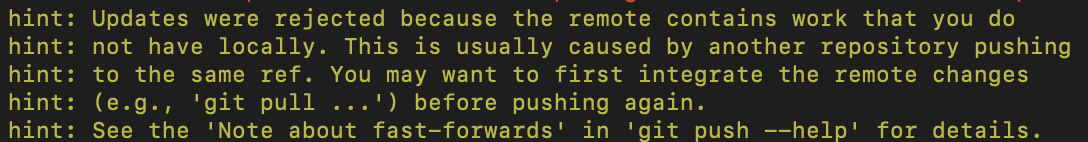
\includegraphics[width=\textwidth]{images/erreur_push_git.png}
    \caption{Message d'erreur quand des modifications ont été faites sur le dépôt git mais pas dans la version locale sur votre ordinateur.}\label{fig:erreur_push_git}
\end{figure}

En effet, après avoir clôner le dépôt, nous avons fait des modifications directement sur GitHub. Puis, nous avons modifié la version locale. Les deux versions n'étant pas identique, il est nécessaire de se mettre-à-jour avant de soumettre nos modifications.

\begin{myexampleblock}{Exercice : Gérer manuellement la fusion}
    \begin{enumerate}
        \item Tapez \texttt{git pull}
        \item Si vous obtenez une erreur similaire à la figure~\ref{fig:erreur_pull_git}, suivez les étapes suivantes :
        \begin{enumerate}
            \item Tapez \texttt{git config pull.rebase false}
            \item Tapez \texttt{git pull}
        \end{enumerate}
        \item Tapez \texttt{git status}.
    \end{enumerate}
\end{myexampleblock}

\begin{figure}[!h]
    \centering
    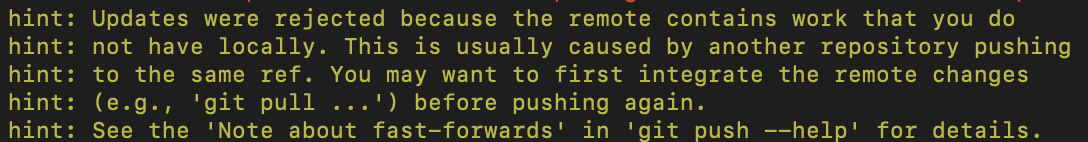
\includegraphics[width=\textwidth]{images/erreur_push_git.png}
    \caption{Message d'erreur quand des modifications ont été faites sur le dépôt git mais pas dans la version locale sur votre ordinateur.}\label{fig:erreur_pull_git}
\end{figure}

Après toutes ces étapes, vous devriez avoir une sortie similaire à celle de la figure~\ref{fig:git_status}

\begin{figure}[!h]
    \centering
    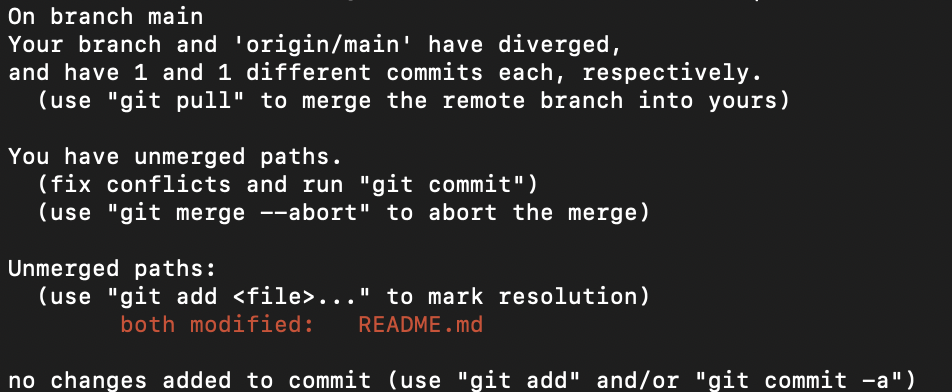
\includegraphics[width=\textwidth]{images/git_status.png}
    \caption{Sortie dans la console après la commande \texttt{git status}.}\label{fig:git_status}
\end{figure}

On voit bien en rouge que les deux branches ont modifiées le README. Nous allons donc ouvrir le README dans votre éditeur de code préféré. Dans le README, vous devriez voir les symboles suivant : \code{<<<<<<<}, \code{=======}, \code{>>>>>>>}, similairement à la figure~\ref{fig:git_merge}.

\begin{figure}[!h]
    \centering
    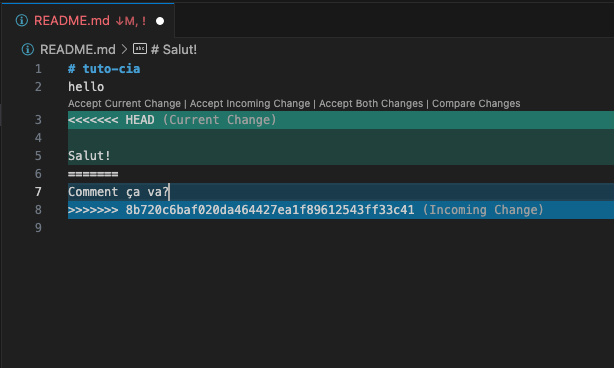
\includegraphics[width=\textwidth]{images/git_merge.png}
    \caption{Apparence du fichier README lorsque la fusion a échoué.}\label{fig:git_merge}
\end{figure}

La section entre \code{<<<<<<<} et \code{=======} correspond au code local en conflit. La section entre \code{=======} et \code{>>>>>>>} correspond au code déjà soumis sur GitHub qui rentre en conflit avec votre code local. Dans la figure~\ref{fig:git_merge}, VSCode propose quatre options pour gérer le conflit. Vous pouvez accepter les modifications locales, accepter les modifications entrantes ou faire un mélange des deux. Si vous savez quelle version choisir, laissez l'éditeur faire son travail et cliquer sur une des deux options. Sinon, vous pouvez manuellement modifier le fichier jusqu'à ce qu'il soit à votre goût. Assurez vous d'enlever les symboles \code{<<<<<<<}, \code{=======}, \code{>>>>>>>}. 

\begin{myexampleblock}{Exercice : Finir la fusion}
    \begin{enumerate}
        \item Ouvrez le fichier README dans un éditeur de code.
        \item Faites les modifications nécessaires. Retirez les symboles associés au conflit. 
        \item Dans le terminal, tapez \texttt{git add README.md}
        \item Tapez \texttt{git commit -m "Mon premier conflit!"}
        \item Tapez \texttt{git push}
    \end{enumerate}
\end{myexampleblock}
Normalement, si tout a fonctionné, les modifications devraient apparaître sur GitHub! 

Pour plus d'information sur les conflits, allez voir ici : \href{https://docs.github.com/fr/pull-requests/collaborating-with-pull-requests/addressing-merge-conflicts/resolving-a-merge-conflict-using-the-command-line}{Lien du tutoriel GitHub}.
\section{Fonctionnalités GitHub}
Normalement, avec tout ce qui a été discuté jusqu'à maintenant, vous devriez être en mesure d'utiliser Git et GitHub. Mais, il existe des fonctionnalités de GitHub dont nous n'avons toujours pas parlé. Par exemple, peut-être vous souviendrez-vous avoir vu, lors de la modification du README sur GitHub, l'option \code{Create a new branch for this commit and start a pull request}. Les branches permettent de travailler sans avoir peur de faire une erreur dans le code. De plus, lors d'un travail d'équipe, cela permet à chacun de développer tranquillement sans gérer de fusion, avant de pousser le tout dans la branche principale. 

Un autre outil utile est la création d'\emph{issues} sur GitHub. Les \emph{issues} GitHub permettent de décrire un problème ou une tâche. 

\subsection{Créer des issues}
Tel que mentionné plus haut, les \emph{issues} sont des tickets de tâches qui devront être accomplies plus tard. Ces tickets contiennent un titre et une description, et peuvent être assigner à un membre du dépôt. 

\begin{myexampleblock}{Exercice : Créer un \emph{issue}}
    \begin{enumerate}
        \item Ouvrez votre dépôt GitHub et ouvrez la section \emph{issues}
        \item Cliquez sur le bouton vert \code{New issue}
        \item Ajoutez un titre. Je recommande ``Mon premier issue''
        \item Ajoutez une courte description.
        \item Dans le coin à droite, assignez vous-même à l'issue.
        \item Créez l'issue
    \end{enumerate}
\end{myexampleblock}
Maintenant que l'\emph{issue} est créé, il sera disponible jusqu'à ce qu'il soit fermé. Dans le cadre de certains gros projets, par exemple \href{https://github.com/scikit-learn/scikit-learn/issues}{Scikit-Learn}, il est possible de reporter un bug ou poser une question. Un \emph{issue} peut être fermé de deux façons différentes : \code{Close as completed} et \code{Close as not planned}. Lorsque vous avez réglé le problème, l'\emph{issue} va être fermée en tant que complétée. Toutefois, si vous ne souhaitez plus réglez le problème, ou c'était une amélioration que vous n'avez pas le temps ou l'envie de faire, vous pouvez fermer l'\emph{issue} en tant que ``non planifié''. 

Après l'ouverture d'une \emph{issue}, GitHub propose automatiquement de créer une branche sur laquelle régler le problème. 

\subsection{Créer une branche}
Nous allons maintenant créer la branche. Sur la branche, vous pouvez faire toutes les modifications en rapport avec le problème que vous résolvez. Lorsque l'\emph{issue} sera réglé, vous pourrez fusionner votre branch avec la branche principale. Créons maintenant la branche. 

\begin{myexampleblock}{Exercice : Créer une branche}
    \begin{enumerate}
        \item Ouvrez l'issue qui vous intéresse
        \item Cliquez sur \code{Create a branch} en bas à droite
        \item Modifiez le nom de l'issue pour un nom un peu plus courte
        \item Sélectionnez \code{Checkout locally}
        \item Cliquez sur le bouton vert \code{Create branch}
    \end{enumerate}
\end{myexampleblock}

Pour accéder à la branche, vous pouvez suivre les instructions de GitHub. 
\begin{myexampleblock}{Exercice : Accéder à la branche}
    \begin{enumerate}
        \item Dans le terminal, tapez \code{\texttt{git fetch origin}}
        \item Entrez \code{\texttt{git checkout <nom-de-la-branche>}}
    \end{enumerate}
\end{myexampleblock}

Modifiez maintenant le README sur la nouvelle branche, puis poussez la modification sur la branche. Nous allons maintenant effectuer un \emph{pull-request}.

\subsection{Pull request}
Les \emph{pull requests} permettent de vérifier les changements qui ont été effectués sur la branche. Elles sont aussi utilisées pour faire vérifier le code par des collègues avant de fusionner les modifications à la branche principale. Vos collègues pourront mettre des commentaires et demander des modifications avant d'accepter la fusion. 

Si vous ne l'avez pas encore fait, faites une modification dans le README sur la nouvelle branche, puis poussez la modification sur la branche. En allant sur GitHub dans la section \code{Pull requests}, vous verrez maintenant un nouveau message disant \code{<nom-de-la-branche> had recent pushes $x$ minutes ago}. Cliquez maintenant sur \code{Compare \& pull request}. 
\begin{myexampleblock}{Exercice : Créer une \emph{pull request}}
    \begin{enumerate}
        \item Cliquez sur \code{Compare \& pull request}
        \item Ajoutez un titre parlant
        \item Ajoutez une courte description de la modification
        \item Cliquez sur le bouton vert \code{Create pull request}
    \end{enumerate}
\end{myexampleblock}

Normalement, si c'était un projet avec plusieurs coéquipiers, vous seriez amener à ajouter des reviewers. Sans l'approbation des reviewers, vous ne serez pas en mesure de fusionner votre code avec la branche principale. De plus, GitHub vous indique s'il y a un conflit avec la branche principale. Dans ce cas, j'utilise généralement \href{https://gist.github.com/whoisryosuke/36b3b41e738394170b9a7c230665e6b9}{ce tutoriel}.

Après la création d'une \emph{pull request}, vous avez accès à la conversation avec les reviewers, les différents \emph{commit} que vous avez poussé sur la branche ainsi qu'une comparaison entre le code sur la branche principale et sur les modifications entrantes. 

Quand le code est approuvé, cliquez sur \code{Merge pull request}. Le code sera maintenant fusionné à la branche principale. GitHub vous proposera de plus de 
supprimer la branche. Puisqu'elle ne sera plus utilisée, généralement, vous pouvez la supprimer immédiatement. En fermant la \emph{pull request}, généralement, l'\emph{issue} va être fermée en tant que complétée. 

\end{document}